\chapter{Risk Management}\label{ch:Risk Management}

Når det gælder software projekter, eller projekter i det hele taget, er der flere risici, som bør identificeres, overvejes og analyseres. Risici er mulige negative afvigelser fra planen.\cite{SlideRiskAnalysis} I dette afsnit, vil gruppen danne et overblik over forskellige metoder, som kan bruges til at identificere risici, samt hvordan risici er blevet analyseret og håndteret i dette projekt.

\section{Risici}

Der er mange mulige metoder til at analysere, hvilke risici et team står overfor. Fælles for dem er, at man starter ud med at identificere mulige risici.
Identificering af ricisi kan blive skåret ned i meget mindre trin.\cite{SlideRiskAnalysis} Disse trin fokuserer på at stille en række spørgsmål til, hvilket slags projekt det er, hvor mange der kommer til at benytte det og hvad der vil ske hvis det ikke virker? Hertil, en reflektion over tidligere projekter - hvilke erfaringer teamet fik, samt hvilke risici der blev fundet. Til sidst, beskrives det i ‘cause, event and effect’. Identificerings processen er i sig selv, en brainstorming process.

Det næste punkt, efterfulgt af at identificere, er vurdering af risici. Vurderingen af risici gennemgår 2 punkter: Estimering, og evaluering. Estimering dækker sandsynligheden for at en risiko kan blive virkelig og hvilken effekt det vil have for både trusler og muligheder. Evaluering er når man samler alle risici og danner en risikoværdi for hele projektet.

\section{Boehm}

Boehm skemaet danner et bedre overblik over det metodevalg, som teamet har taget. Da det ikke altid er den agile metode, der er det bedste valg til et projekt er det vigtigt at identificere hvilke risici, der kan opstå ved netop at benytte den agile tilgang. En fejl teamet kan begå, er eksempelvis at automatisk gå ud fra, at en agil tilgang er det bedste valg. For at finde det bedste valg for dette projekt, har vi benyttet Boehm skemaet, til at finde hvor gruppen ligger på skemaet, og hvilken metode der kan vælges ud fra skemaet.
Teamet er på 4 personer så størrelsen på personel er meget lille, så disse to punkter er tættere på midten af skemaet. Vi er i et meget behageligt projekt, da hvis noget går galt, vil det for det første hverken koste et eller flere liv, men det vil heller ikke påvirke økonomisk status, beboelses status eller fysisk helbred. Kigger vi i det hele taget på Boehm skemaet, bliver det hurtigt tydeligt, at teamet falder ind under de røde linjer og derfor den agile tilgang være fordelagtig.

\begin{figure}
    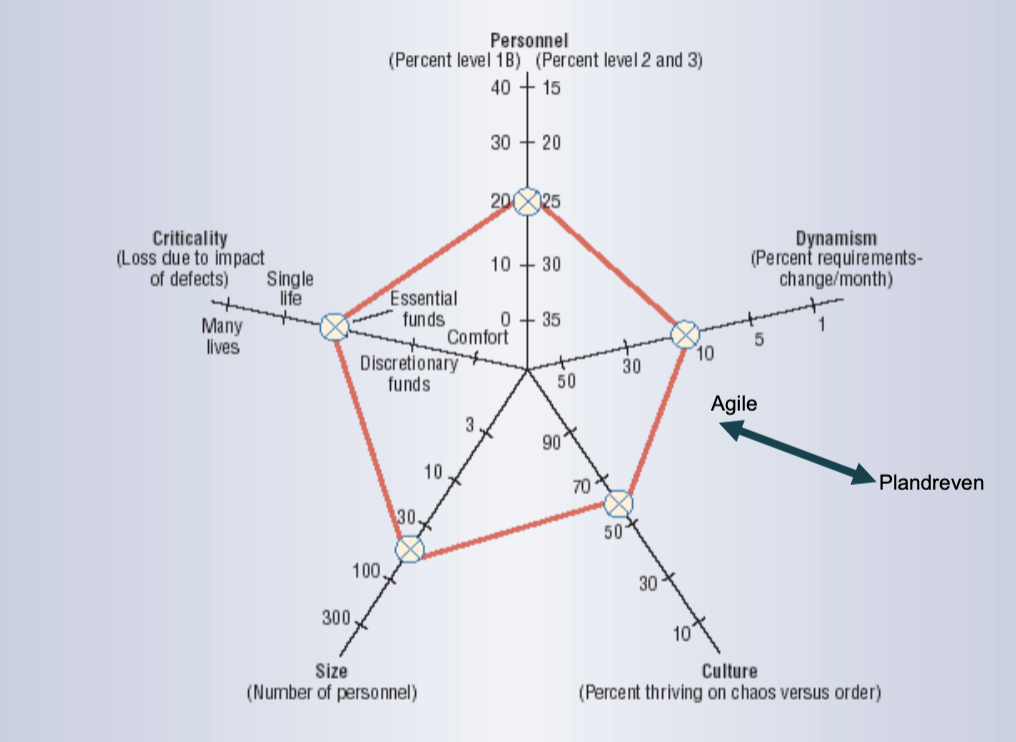
\includegraphics[width=\linewidth]{figures/Boehm.png}
    \caption{Boehm's kritiske faktor.}
    \label{fig:Boehm}
\end{figure}

\section{Identificerede risici}\label{sec:identified_risks}
\begin{figure}
    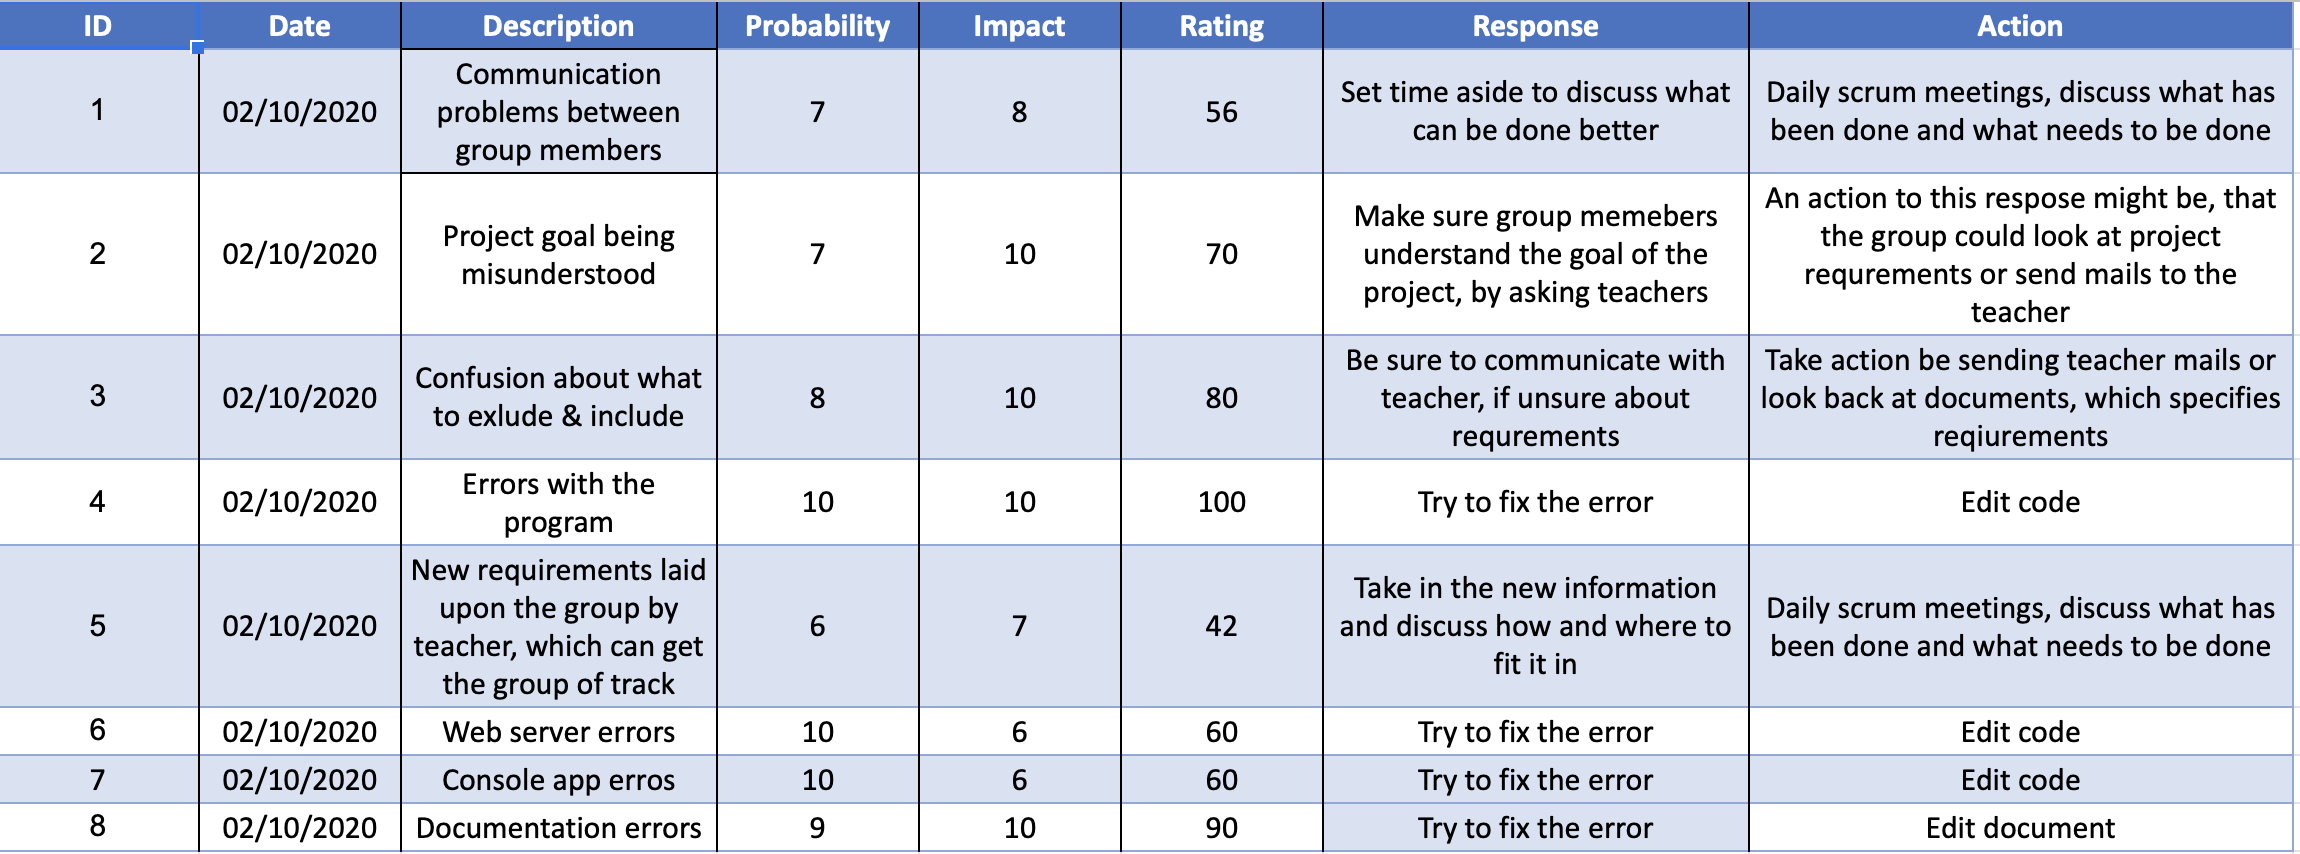
\includegraphics[width=\linewidth]{figures/RiskRegister.png}
    \caption{Teamets Risk Register}
    \label{fig:Risk}
\end{figure}
På figur \ref{fig:Risk} er der dannet et risk register til dette projekt. Før oprettelsen af denne risk register, har teamet, som det første identificeret risici, som er beskrevet under ‘Description’. Dette blev gjort ved brug af brainstorming og erfaringer fra tidligere projekter. Efterfølgende har teamet vurderet risici, ved at gennemtænke sandsynligheden for hver risiko og hvilken indvirkning det ville have på projektet. Når både sandsynligheden og indvirkningen er vurderet, kan de rangeres ved at gange de to. Til sidst har gruppen gennemtænkt det bedste respons til hver risiko, med en kort beskrivelse. Der står beskrevet hvad teamet skal gøre såfremt en risiko opstår. 

Med dette, er det vigtigt at sørge for projektet ikke bare er sikkert, men også af god kvalitet. Som vi vil kigge nærmere på, når vi har været igemmen hvordan arkitekturen er opsat. 


\section{Håndtering af risici}\label{sec:handling_risks}
Ikke alle risici kom op i dette projekt, men de som blev relevante skulle håndteres på gruppen. De risici fra figur \ref{fig:Risk}, der blev relevante, er:
\begin{itemize}
    \item Kommunikationsproblemer mellem gruppemedlemmer
    \item Forvirring om hvad der skal inkluderes og ekskluderes fra projektet
    \item Fejl i programmet
    \item Dokumentationsfejl
\end{itemize}

Kommunikationsproblemerne opstod i form af at ét eller flere gruppemedlemmer var fraværende til enkelte morgenmøder. Dette gjorde at motivationen for at arbejde var svækket, men problemerne blev håndteret ved at følge op på hinanden senere på dagen, og at alle fik arbejdet på projektet til trods for fravær. 
Hver gang der opstod forvirring omkring hvad rapporterne skulle indeholde, blev der snakket i gruppen om, hvad vi selv mente, og vi hjalp hinanden med at finde ressourcer til struktur og indhold af rapporten, samt fik skrevet mails til vejledere med spørgsmål.
Fejl i programmet blev altid rapporteret til resten af gruppen, og senere løst af et andet gruppemedlem. Dette betød at fejl i programmet blev løst før de blev glemt eller udeladt. 
Dokumentationsfejl opstod tidligt i projektet, da flere gruppemedlemmer havde svært ved at få rapporten til at fungere. 
Udover de forventede risici opstod der også problemer med planlægning af kapacitet til hvert sprint. Der blev under beregningen af kapaciteten ikke modregnet weekender, fritidsarbejde eller private ærinder. Dette betød at der i løbet af pre-sprint, sprint \#0 og sprint \#1 var for mange opgaver som skulle løses ift. hvor meget tid der var til at lave dem. I sprint \#2 og \#3 blev kapaciteten beregnet ud fra erfaringer fra tidligere sprint og modregninger blev også håndteret bedre. Det lykkedes så at komme i mål med sprint \#2 %og 3?
%TODO: write a bit about sprint #3